\documentclass[11pt]{scrartcl}

\usepackage[utf8]{inputenc} 
\usepackage[T1]{fontenc}     
\usepackage[french]{babel} 
\usepackage{lmodern}
\usepackage{microtype}
\usepackage{xcolor}
\usepackage{sectsty}
\usepackage{geometry} 
\usepackage{fancyhdr}  
\usepackage{graphicx}        
\usepackage{amsmath, amssymb} 
\usepackage[hidelinks]{hyperref} 

\hypersetup{pdfnewwindow=true}
\definecolor{mainblue}{RGB}{0, 102, 204}
\setcounter{secnumdepth}{0}   
\sectionfont{\color{blue!60!black}\sffamily\Large\bfseries}  
\geometry{margin=2cm}


%%%%%%%%%%%%%%%%%%%%%%%%%%%%%%%%%%%%%%%%%%%%%%%%%%%%%%%%%%%%%%%%%%%%%%%%%%%%%%%%%%%%%%%
%%%%%%%%%%                       EN-TÊTE ET PIED DE PAGE                     %%%%%%%%%%
%%%%%%%%%%%%%%%%%%%%%%%%%%%%%%%%%%%%%%%%%%%%%%%%%%%%%%%%%%%%%%%%%%%%%%%%%%%%%%%%%%%%%%%

\pagestyle{fancy}
\fancyhf{} 

%%% En-tête de page
\fancyhead[L]{\footnotesize IUT de Lannion - Département Informatique}
\fancyhead[R]{\footnotesize 2025} 

%%% Pied de page
\fancyfoot[L]{\footnotesize © Stanislas ROLLAND - Pierre LECHAT - Tous droits réservés} 
\fancyfoot[R]{\footnotesize \thepage}

\renewcommand{\footrulewidth}{0.4pt}


%%%%%%%%%%%%%%%%%%%%%%%%%%%%%%%%%%%%%%%%%%%%%%%%%%%%%%%%%%%%%%%%%%%%%%%%%%%%%%%%%%%%%%%
%%%%%%%%%%                        PAGE DE PRÉSENTATION                       %%%%%%%%%%
%%%%%%%%%%%%%%%%%%%%%%%%%%%%%%%%%%%%%%%%%%%%%%%%%%%%%%%%%%%%%%%%%%%%%%%%%%%%%%%%%%%%%%%

\title{Rapport d'analyse de données - Joueurs de football}
\author{Stanislas ROLLAND - Pierre LECHAT}
\date{Septembre 2025}

\begin{document}

    \maketitle
    \tableofcontents  
    \newpage
 

    %%%%%%%%%%%%%%%%%%%%%%%%%%%%%%%%%%%%%%%%%%%%%%%%%%%%%%%%%%%%%%%%%%%%%%%%%%%%%%%%%%%
    %%%%%%%%%%                          INTRODUCTION                         %%%%%%%%%%
    %%%%%%%%%%%%%%%%%%%%%%%%%%%%%%%%%%%%%%%%%%%%%%%%%%%%%%%%%%%%%%%%%%%%%%%%%%%%%%%%%%%

    \section{Introduction}

    Dans le cadre de ce travail, nous nous intéressons à l’analyse statistique d’un jeu de données regroupant les performances de joueurs de football évoluant dans les cinq grands championnats européens (Premier League, La Liga, Serie A, Bundesliga et Ligue 1) pour la saison 2024--2025. 
    L’objectif principal de cette analyse est de dégager des tendances et des profils types parmi les joueurs, en tenant compte à la fois de leurs statistiques individuelles (buts, passes décisives, temps de jeu, etc.) et de leurs caractéristiques qualitatives (poste, équipe, nationalité, etc.). Pour ce faire, nous avons choisi d’appliquer deux techniques complémentaires d’analyse de données :
    \begin{itemize}

        \item \textbf{L’Analyse en Composantes Principales (ACP)} : une méthode d’analyse multivariée appliquée aux données quantitatives, permettant de réduire la dimensionnalité tout en conservant un maximum d’information. Elle nous aidera à visualiser les relations entre les différentes variables numériques et à identifier des profils de joueurs.  
        \item \textbf{Une méthode d’analyse de données qualitatives} : qui permettra de mettre en valeur les variables catégorielles (poste, compétition, équipe, etc.) et de mieux comprendre la répartition des joueurs selon leurs caractéristiques.  
    
    \end{itemize}
    En combinant ces deux approches, nous espérons obtenir une vision globale et nuancée des performances des joueurs de football, en tenant compte à la fois de leurs statistiques individuelles et de leur contexte compétitif. Ce rapport détaillera les étapes de notre analyse, les résultats obtenus, ainsi que les interprétations que nous en tirerons.


    %%%%%%%%%%%%%%%%%%%%%%%%%%%%%%%%%%%%%%%%%%%%%%%%%%%%%%%%%%%%%%%%%%%%%%%%%%%%%%%%%%%
    %%%%%%%%%%                         JEU DE DONNÉES                        %%%%%%%%%%
    %%%%%%%%%%%%%%%%%%%%%%%%%%%%%%%%%%%%%%%%%%%%%%%%%%%%%%%%%%%%%%%%%%%%%%%%%%%%%%%%%%%

    \section{Présentation du jeu de données}

        \subsection{Description du jeu de données}
        Le jeu de données que nous avons choisi d'analyser est un ensemble de données concernant les statistiques des joueurs de football sur la saison 2024 - 2025 les cinq meilleures ligues européennes (Premier League, La Liga, Serie A, Ligue 1, Bundesliga).\\\\
        Notre jeu de données comporte 197 entrées (une par joueur) et les 15 variables suivantes :

        \textbf{\\\underline{Variables qualitatives :}\\}
            \begin{itemize}

                \item \textbf{Player} : Nom et prénom du joueur.
                \item \textbf{Nation} : Nationalité du joueur.
                \item \textbf{Pos} : Position principale du joueur sur le terrain (ex : Attaquant, Défenseur, Gardien).
                \item \textbf{Squad} : Équipe actuelle du joueur.
                \item \textbf{Comp} : Compétition dans laquelle le joueur évolue (ex : Premier League, La Liga etc).
                
            \end{itemize}
        
        \textbf{\\\underline{Variables quantitatives :}\\}
            \begin{itemize}

                \item \textbf{Id} : Identifiant unique du joueur.
                \item \textbf{Age} : Âge du joueur.
                \item \textbf{Born} : Année de naissance du joueur.
                \item \textbf{MP} : Nombre de matchs joués par le joueur.
                \item \textbf{Starts} : Nombre de matchs commencés comme titulaire.
                \item \textbf{Min} : Nombre total de minutes jouées.
                \item \textbf{90s} : Nombre de périodes de 90 minutes jouées (équivalent à des matchs complets).
                \item \textbf{Gls} : Nombre total de buts marqués.
                \item \textbf{Ast} : Nombre total de passes décisives.
                \item \textbf{G+A} : Somme des buts et des passes décisives.
            
            \end{itemize}

        \subsection{\\Exemple d'une entrée du jeu de données\\}

        \begin{center}

            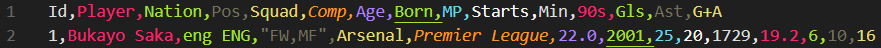
\includegraphics[width=1\textwidth]{images/exemple_entree.png}
            \captionof{figure}{}

        \end{center}    



    %%%%%%%%%%%%%%%%%%%%%%%%%%%%%%%%%%%%%%%%%%%%%%%%%%%%%%%%%%%%%%%%%%%%%%%%%%%%%%%%%%%
    %%%%%%%%%%               TECHNIQUES D'ANALYSE DE DONNÉES                 %%%%%%%%%%
    %%%%%%%%%%%%%%%%%%%%%%%%%%%%%%%%%%%%%%%%%%%%%%%%%%%%%%%%%%%%%%%%%%%%%%%%%%%%%%%%%%%

    \section{Les techniques d'analyse de données}

    \subsection{Analyse quantitative des données : l'ACP}
    \subsection{Analyse catégorielle / qualitative des données : la CAH}


    %%%%%%%%%%%%%%%%%%%%%%%%%%%%%%%%%%%%%%%%%%%%%%%%%%%%%%%%%%%%%%%%%%%%%%%%%%%%%%%%%%%
    %%%%%%%%%%                            CONCLUSION                         %%%%%%%%%%
    %%%%%%%%%%%%%%%%%%%%%%%%%%%%%%%%%%%%%%%%%%%%%%%%%%%%%%%%%%%%%%%%%%%%%%%%%%%%%%%%%%%

    \section{Conclusion}


\end{document}